%%%%%%%%%%%%%%%%%%%%%%%%%%%%%%%%%%%%%%%%%%%%%%%%%%%%%%%%%%%%%%%%%%%%%%%%%%%%%%%
\chapter{Flusso su corpi}\label{chp:FlowBodieas}
%%%%%%%%%%%%%%%%%%%%%%%%%%%%%%%%%%%%%%%%%%%%%%%%%%%%%%%%%%%%%%%%%%%%%%%%%%%%%%%

Un fluido in movimento apporta forze di pressione normali ad un corpo immerso e forse tangenziali alla superficie.
Per un flusso bidimensionale, la risultante della pressione e forze di taglio possono essere considerate in due componenti:
\begin{itemize}
\item \eng{Drag force} in direzione del flusso;
\item \eng{Lift force} in direzione normale al flusso.
\end{itemize}
Nel caso di un flusso tridimensionale c'è una componente mista normale al piano \eng{drag-lift}.
Allora, le forze possono generare anche dei momenti come:
\begin{itemize}
\item momento di rollio,
\item momento di beccheggio,
\item momento di bardata.
\end{itemize}

\begin{equation}
\begin{split}
F_D &= \int_A{\left(-p\cos\theta + \tau_W\sin\theta\right)\,dA}\\
F_L &= -\int_A{\left(p\sin\theta + \tau_W\cos\theta\right)\,dA}
\end{split}
\end{equation}

\begin{figure}
\centering
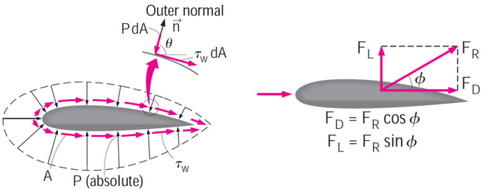
\includegraphics[width = \textwidth]{gfx/DragLift}
\caption{Scomposizione delle forze su un profilo alare in \eng{drag} e \eng{lift}}
\label{fig:DragLift}
\end{figure}

Sia la frizione superficiale sia la pressione, in generale, contribuiscono a $F_D$ e $F_L$. In caso di una lastra piana fina allineata parallela alla direzione del flusso, $F_D$ dipende solamente dalle forze di taglio.
Quando la lastra è normale alla direzione del flusso $F_D$ dipende solo dalla pressione.

\section{Coefficienti di drag e lift}
i coefficienti di \eng{drag} e \eng{lift} sono definiti come:
\begin{equation}
C_D = \frac{F_D}{\rho \frac{V^2}{2}A} \qquad C_L = \frac{F_L}{\rho \frac{V^2}{2}A}
\end{equation}
I due coefficienti rappresentano il comportamento di \eng{drag} e \eng{lift} del corpo.
In generale dipendo dalle caratteristiche geometriche del corpo. Dipendono anche dal numero di Reynolds e dalla rugosità della superficie.
I coefficienti locali, variano lungo la superficie in finzione dei cambiamenti della velocità dello strato limite nella direzione di flusso.
Si può definire i coefficienti medi del corpo nel momento in cui sono disponibili i coefficienti locali lungo tutta la lunghezza della superficie. 
Possono dipendere anche dal numero di Mach, a patto che sia rilevante per la geometria: $Ma \geq 0.3$.

\subsection{Composizione drag}
La forza di \eng{drag} è composizione di diversi fenomeni:
\begin{description}
\item[Frizione] dovuta prevalentemente dagli sforzi di taglio sulla parete $\tau_W$. Causata da effetti d'attrito.
\item[Pressione] dovuta al contributo della pressione sul profilo. Definita anche dalla forte dipendenza dalla geometria del corpo.
\end{description}
Si può definire:
\begin{equation}
F_D = F_{D, \textup{Friction}} + F_{D, \textup{Pressure}} \qquad C_D = C_{D, \textup{Friction}} + C_{D, \textup{Pressure}}
\end{equation}

La $F_{D,\textup{friction}}$ è una funzione importante legata alla viscosità: aumenta con l'aumentare della viscosità. In particolare , per flussi a basso numero di Reynolds la maggior parte del \eng{drag} è dovuto alla frizione.
Con l'aumentare del numero di Reynolds il \eng{drag} per effetto della frizione cala.
$F_{D,\textup{friction}}$ è proporzionale all'area della superficie. 
$C_{D,\textup{friction}}$ è indipendente dalla rugosità superficiale nel flusso laminare, è fortemente dipendente dalla rugosità superficiale nel caso di flussi turbolenti.
$F_{D,\textup{pressure}}$ è proporzionale all'area frontale e alle differenze di pressione tra il fronte e il retro del corpo immerso. È dominante per i corpi spuntati risulta piccolo per corpi affusolati come ad esempio i profili alari e nullo nel caso di lastre piane parallele al flusso.
$F_{D,\textup{pressure}}$ Risulta molto significativo quando la velocità del fluido è molto alta e quest'ultimo è capace di seguire la curvatura del corpo. Perciò il fluido quando si separa dal corpo crea un gradiente di pressione molto basso nel retro del corpo stesso.

\paragraph{Ridurre il drag: affusolando}
Affusolare un corpo ha degli effetti contrari nel \eng{drag} di pressione e frizione: Riduce il \eng{pressure drag} eliminando la separazione dello strato limite. Mentre aumenta il \eng{friction drag} aumentando l'area della superficie del corpo.
Infatti, spesso vengono condotti degli studi di ottimizzazione del \eng{drag} per far sì che un corpo immerso in un flusso abbia il minimo della somma dei due componenti.
Affusolare dovrebbe essere preso in considerazione per corpi spuntati che sono sottoposti a un flusso ad alto numero di Reynolds, per cui la separazione del flusso è una possibilità reale 

\begin{figure}
\centering
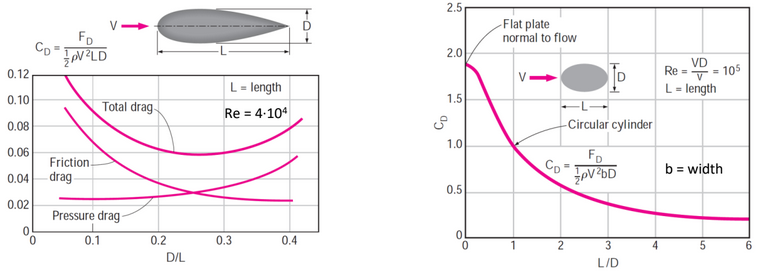
\includegraphics[width = \textwidth]{gfx/Affusolamento}
\caption{Processo di affusolamento di un corpo immerso in un fluido}
\label{fig:Affusolamento}
\end{figure}

In letteratura esistono alcune tabelle che mostrano i coefficienti di \eng{drag} per delle geometrie piuttosto semplici.
Bisogna sempre considerare che oltre alla geometria è molto importante il flusso nella sua composizione, nella velocità e nella sua direzione.

\section{Flusso parallelo ad una lastra piana}
Per una lastra piana parallela al flusso il coefficiente di \eng{drag} è uguale al coefficiente di \eng{drag} per frizione.
Il coefficiente di frizione varia lungo tutta la superficie come risultato dei cambiamenti della velocità all'interno dello strato limite nella direzione del flusso.
I valori del coefficiente di frizione sono molto più alti in un flusso turbolento rispetto a quelli di un flusso laminare; questo è dovuto al fatto che: nel flusso turbolento c'è un maggiore mescolamento rispetto che a quello laminare.

\begin{equation}
F_D = F_{D,\textup{friction}} = F_f = C_f \rho \frac{V^2}{2}A
\label{eqn:DragFriction}
\end{equation}

\begin{figure}
\centering
\subfloat[][]
{%
\begin{minipage}[b]{0.4\textwidth}
\textbf{Per un flusso laminare}, il $C_f$ dipende solamente dal numero di Reynolds e la rugosità della superficie non ha effetto.
\textbf{Per un flusso turbolento}, la rugosità della superficie causa l'incremento considerevole del $C_f$ a tal punto che un regime completamente turbolento è funzione della sola rugosità e non del numero di Reynolds
\end{minipage}%
} \quad
\subfloat[][\emph{$C_f$ in funzione del numero di Reynolds e della rugosità $\epsilon$}\label{fig:Cf}]
{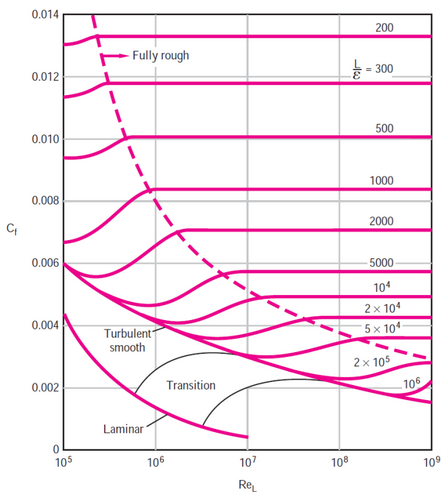
\includegraphics[width = 0.4\textwidth]{gfx/Cf}}
\end{figure}

\section{Flusso su una sfera o un cilindro}
Ipotizzando di considerare una sfera o un cilindro una misura caratteristica di entrambi può essere il diametro $D$.
Da cui si può considerare il numero di Reynolds 
\begin{equation}
Re = \frac{VD}{v}
\end{equation} 
Possiamo considerare il fatto che il numero di Reynolds critico sia $Re_{\textup{cr}} \approx 2*10^5$.
Allora la forza di \eng{drag} sarà inizialmente dovuta alla frizione per numeri di Reynolds bassi. Dopodiché, all'aumentare del numero di Reynolds, inizierà il contributo di entrambe le componenti fino ad arrivare interamente al contributo della sola componente pressoria.
Il fenomeno può essere descritto in funzione del numero di Reynolds:
\begin{description}
\item[$Re < 10^3$]Per numeri di Reynolds estremamente bassi gli effetti dell'inerzia sono trascurabili e il fluido copre totalmente il corpo. Non cè separazione del flusso e il coefficiente di \eng{drag} è inversamente proporzionale al numero di Reynolds. Salendo col numero di Reynolds inizia la separazione del flusso nella parte posteriore del corpo. Mentre, il coefficiente di \eng{drag} continua a decrescere con l'aumento del numero di Reynolds. 
\item[$10^3 < Re < 10^5$] Per questa velocità il coefficiente di \eng{drag} rimane più o meno costante. Questo comportamento è caratteristico dei corpi spuntati. Il flusso nello strato limite è laminare in questo range, ma il flusso della regione separata, dopo il corpo, è fortemente turbolento con una larga scia vorticosa.
\item[$Re > 10^5$]Dopo questo pallone limite il coefficiente di \eng{drag} subisce un'improvvisa caduta. Questo è dovuto al fatto che lo strato limite diventa turbolento. Allora il punto di distacco tra lo strato limite e il corpo si sposta sul retro del corp,o riducendo la dimensione della scia e la magnitudo della \eng{drag} di pressione. 
\end{description} 

Un incremento della rugosità superficiale può diminuire il $C_f$. Ciò è dovuto  alla transizione dello strato limite da valori laminari a quelli turbolenti causando nel flusso posteriore al corpo una riduzione della scia e del \eng{drag} di pressione . 

%*****************************************
\chapter{Aerodinamica di un profilo alare}\label{ch:Airfoil}
%*****************************************

Al fine di risolvere un flusso sopra un profilo alare, si considera il fatto che valga la sovrapposizione degli effetti.
Così possiamo risolvere attraverso Laplace il flusso, considerando separatamente la funzione velocità potenziale e la \eng{stream function}.
Per ottenere un flusso più complicato, lo si può considerare come somma di flussi elementari.
\begin{equation}
\textup{Flusso uniforme} + \textup{Fonte uscita linee} + \textup{Vortici} = \textup{Flusso complesso}
\end{equation}

\paragraph{Flussi semplici: fonte lineare}
Considerando un flusso bidimensionale che emerge da una fonte su un piano $xy$ e disperdendosi in maniera radiale in tutte le direzioni con un rateo di flusso totale per profondità $q \left[\unit{\m^2/s}\right]$.
Allora le equazioni di conservazione della massa:
\begin{equation}
q = (2\pi r)V_r \quad V_r = q/2\pi r \quad V_{\theta} =0
\end{equation}
Nell'origine è presente una singolarità matematica per cui la velocità non è definita.
Viene rappresentato alla figura \ref{fig:LinearSource}.

\begin{figure}
\centering
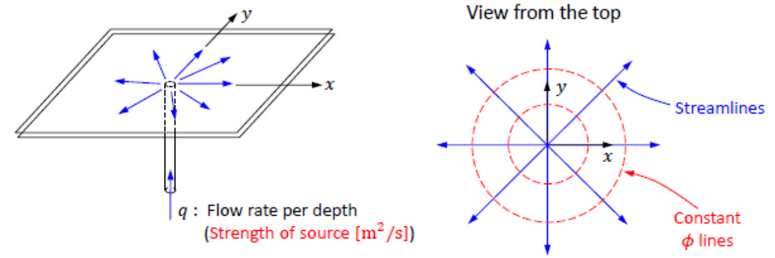
\includegraphics[width = \textwidth]{gfx/LinearSource}
\caption{Fonte lineare}
\label{fig:LinearSource}
\end{figure}

Allora ne calcoliamo la funzione potenziale:
\begin{equation}
V_r = \frac{\partial \phi}{\partial r} \Rightarrow \frac{q}{2\pi r} = \frac{\partial \phi}{\partial r} \Rightarrow \phi = \frac{q}{2\pi}\ln(r) + f(\theta)
\end{equation}
\begin{equation}
V_{\theta} = \frac{1}{r}\frac{\partial \phi}{\partial \theta} \Rightarrow 0 = \frac{1}{r}\frac{df}{d\theta} \Rightarrow \frac{df}{d\theta} = 0
\end{equation}
Ne risulta che $f$ è costante.
Dunque:
\begin{equation}
\phi = \left(\frac{q}{2\pi}\right)\ln(r)
\end{equation}

\paragraph{Vortice libero}
Il concetto di vortice libero è già stato introdotto al capitolo \ref{chp:RotIrrotFlow} a pagina \pageref{chp:RotIrrotFlow}.

Importante ricordare che la vorticità di un vortice libero è sempre nulla ad eccezione dell'origine che è una singolarità matematica.

\paragraph{Circuitazione}
La forza di un vortice non è misurata dalla costante $K$ che definisce la funzione del vortice \eqref{eqn:FreeVortex} a pagina \pageref{eqn:FreeVortex}, bensì la sua circuitazione $\Gamma$.
La circuitazione è la linea integrale della componente tangenziale del vettore velocità attorno ad una curva chiusa. Viene relazionata con la rotazionalità del flusso.

\begin{figure}
\centering
\subfloat[][\emph{Parametri dell'integrale di circuitazione}\label{fig:Circuitazione}]
{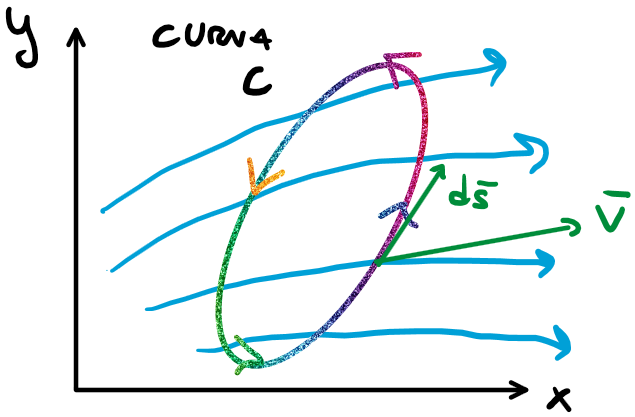
\includegraphics[width = 0.4\textwidth]{gfx/Circuitazione}}\quad
\subfloat[][\emph{Definizione circuitazione}\label{def:Circuitazione}]
{%
\begin{minipage}[b]{0.4\textwidth}
\begin{equation}
\Gamma = \oint_C \vec{V} \,d\vec{s} \quad \left[m^2/s\right]
\label{eqn:Circuitazione}
\end{equation}
Dove:\\
\begin{tabular}{cp{0.9\textwidth}}
$C$ & rappresenta la linea in cui viene calcolata la circuitazione\\
$\vec{s}$ & vettore differenziale lungo il percorso di integrazione
\end{tabular}\\
\end{minipage}%
}
\caption{Descrizione della circuitazione su una curva immersa in un campo}
\end{figure}

Vortici irrotazionali sono irrotazionali ovunque ad eccezione dell'origine. Tutta la circuitazione è concentrata all'interno dell'origine. Infatti, è un punto singolare.

Allora, la circuitazione per il vortice libero risulta essere:
\begin{equation}
\Gamma = 2\pi K
\label{eqn:CircFreeVortex}
\end{equation}

\section{Circuitazione di una fonte lineare e campo di flusso uniforme}
Una fonte puntuale ha circuitazione nulla su qualsiasi circuito.
La proprietà di circuitazione nulla di una fonte planare, ha importanti conseguenze nella rappresentazione del flusso.
Qualsiasi modello aerodinamico consiste nella combinazione di un campo di flusso uniforme e una fonte planare che abbia $\Gamma = 0$.

\begin{figure}
\centering
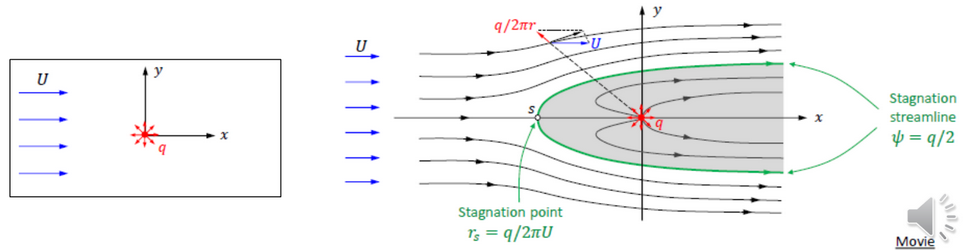
\includegraphics[width = \textwidth]{gfx/ComboFlussoFonte}
\caption{Combinazione tra flusso uniforme e fonte planare}
\label{fig:ComboFlussoFonte}
\end{figure}

\section{La condizione di Kutta}
Doppiette in presenza di un flusso uniforme:
\begin{enumerate}
\item Prendiamo il caso più semplice di doppietta fonte-pozzo con flusso uniforme nullo: \ref{def:FontePozzo}.
Entrambi agenti sull'origine
\item Complicando ulteriormente, aggiungiamo un flusso a velocità uniforme.
\end{enumerate}

\begin{figure}
\centering
\subfloat[][\emph{Fonte-pozzo flusso nullo}\label{fig:FontePozzo}]
{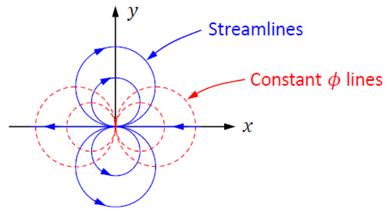
\includegraphics[width = 0.4\textwidth]{gfx/FontePozzo}} \quad
\subfloat[][\emph{Ipotesi}\label{hyp:FontePozzo}]
{%
\begin{minipage}[b]{0.4\textwidth}
\begin{itemize}
\item una fonte di portata $q$ sull'origine.
\item un pozzo di portata $q$ sull'origine.
\end{itemize}
\end{minipage}%
}\\
\subfloat[][\emph{Fonte-pozzo e flusso a velocità uniforme}\label{fig:FontePozzoStream}]
{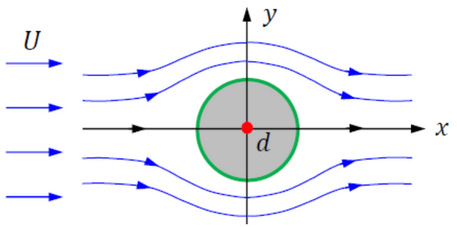
\includegraphics[width = 0.4\textwidth]{gfx/FontePozzoStream}}\quad
\subfloat[][\emph{Ipotesi}\label{hyp:FontePozzoStream}]
{%
\begin{minipage}[b]{0.4\textwidth}
\begin{itemize}
\item una doppietta di portata $d$ sull'origine.
\item flusso a magnitudo costante $U$ in direzione positiva
\end{itemize}
\end{minipage}%
}
\caption{Fonte-Pozzo}\label{def:FontePozzo}
\end{figure}

Ne risulta un comportamento simile a quello del caso della sfera liscia immersa nel fluido a velocità costante.
Si genera una \eng{streamline} nulla detta \eng{stagnation stream line}.
